
\de{ĐỀ THI HỌC KỲ I NĂM HỌC 2022-2023}{THPT Bình Hưng Hòa}


%---Câu 1
\begin{bt}%[0T3Y1-2]%[Dự án đề kiểm tra HKI NH22-23-Thầy Hóa]%[THPT Bình Hưng Hòa]
Tìm tập xác định của các hàm số sau:
\begin{listEX}[2]
	\item $ \dfrac{1+x}{x^2-5x} $
	\item $ \sqrt{2x+4}+\dfrac{x}{\sqrt{6-x}} $
\end{listEX}
\dapso{a) $ D=\mathbb{R}\setminus\left\{0; 5\right\} $; b) $ D=[-2;6) $.}
\loigiai{
\begin{enumerate}
	\item Điều kiện xác định: $x^2-5x\neq 0\Leftrightarrow\heva{&x\neq 0\\&x\neq 5.}$\\
	Vậy tập xác định của hàm số là $\mathscr{D}=\mathbb{R}\setminus \{0;5\}$.
	\item Điều kiện xác định: $\heva{&2x+4\geq 0\\&6-x>0}\Leftrightarrow\heva{&x\geq -2\\&x<6}\Leftrightarrow -2\leq x<6$.\\
	Vậy tập xác định của hàm số là $\mathscr{D}=[-2;6)$.
\end{enumerate}
}
\end{bt}

%---Câu 2
\begin{bt}%[0T3B2-3]%[Dự án đề kiểm tra HKI NH22-23-Thầy Hóa]%[THPT Bình Hưng Hòa]
Lập bảng biến thiên và vẽ đồ thị hàm số $ y=x^2-4x+1 $.
\loigiai{
\immini{
Ta có $\dfrac{-b}{2a}=\dfrac{4}{2}=2$;\\
Với $x=2\Rightarrow y=2^2-4\cdot 2+1=-3$.\\
Suy ra đỉnh $I(2;-3)$.\\
Trục đối xứng $x=2$.\\
Bảng giá trị
\begin{center}
	\begin{tabular}{|c|c|c|c|c|c|}
		\hline $x$ &$0$ &$1$ &$2$ &$3$ &$4$\\
		\hline $y=x^2-4x+1$ &$1$ &$-2$ &$-3$ &$-2$ &$1$\\
		\hline
	\end{tabular}
\end{center}
Vì $a=1>0$ nên đồ thị hàm số $y=x^2-4x+1$ là parabol có bề lõm quay lên.
}{
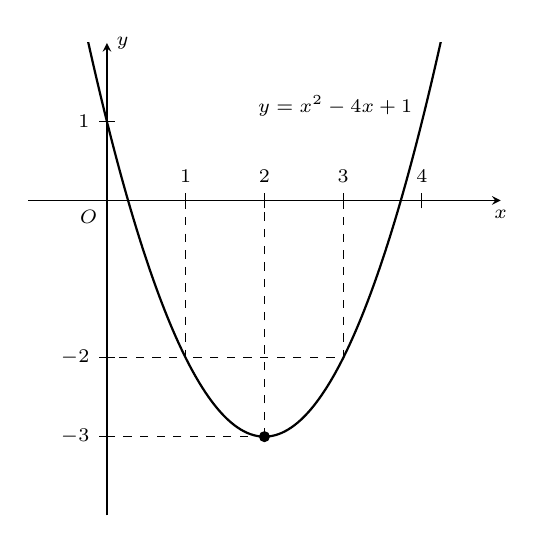
\begin{tikzpicture}[>=stealth,x=1cm,y=1cm,scale=1]
	\def\a{1} % Hệ số a phải khác 0
	\def\b{-4}
	\def\c{1}
	\draw[->] (-1,0) -- (5,0) node[below] {\scriptsize $x$};
	\draw[->] (0,-4) -- (0,2) node[right] {\scriptsize $y$};
	\draw (0,0)node[below left]{\scriptsize $O$};
	\pgfmathsetmacro\xdinh{-(\b)/2*(\a)}
	\pgfmathsetmacro\ydinh{(4*(\a)*(\c)-(\b)^2)/(4*(\a))}
	\fill[dashed] (\xdinh,\ydinh)circle(2pt) edge (\xdinh,0) edge (0,\ydinh);
	\clip (-1,-4)rectangle(5,2);
	\draw[thick,samples=150,smooth,domain=-1:5] plot(\x,{\a*(\x)^2+(\b)*\x+(\c)})node[below left]{\scriptsize $y=x^2-4x+1$};
	\foreach \x in {1,2,3,4}{\draw (\x,-0.1)--++(90:0.2)node[above]{\scriptsize $\x$};}
	\foreach \y in {-2,-3,1}{\draw (0.1,\y)--++(180:0.2)node[left]{\scriptsize $\y$};}
	\draw[dashed] (1,0)|-(0,-2) (3,0)|-(1,-2);
	\node[left] at (4,1.2){\scriptsize $y=x^2-4x+1$};
\end{tikzpicture}
}	
}
\end{bt}

%---Câu 3
\begin{bt}%[0T3B2-2]%[Dự án đề kiểm tra HKI NH22-23-Thầy Hóa]%[THPT Bình Hưng Hòa]
Xác định parabol $ (P)\colon y=ax^2+bx+c $ biết $ (P) $ có đỉnh $ S(1;6) $ và đi qua điểm $ A(-2;3) $.
\dapso{$ y=-\dfrac{1}{3}x^2+\dfrac{2}{3}x+\dfrac{17}{3}$.}
\loigiai{
Ta có $A\in (P)\Rightarrow a\cdot (-2)^2+b\cdot (-2)+c=3\Leftrightarrow 4a-2b+c=3$.\hfill(1)\\
Lại có $S\in(P)\Rightarrow a\cdot 1^2+b\cdot 1+c=6\Leftrightarrow a+b+c=6$.\hfill(2)\\
Hoành độ đỉnh: $\dfrac{-b}{2a}=1\Leftrightarrow 2a+b=0$.\hfill(3)\\
Từ (1), (2) và (3) ta được hệ phương trình
\[\heva{&4a-2b+c=0\\&a+b+c=0\\&2a+b=0}\Leftrightarrow \heva{&a=\dfrac{-1}{3}\\&b=\dfrac{2}{3}\\&c=\dfrac{17}{3}.} \]
Vậy $ y=-\dfrac{1}{3}x^2+\dfrac{2}{3}x+\dfrac{17}{3}$.
}
\end{bt}

%---Câu 4
\begin{bt}%[0T6B2-4]%[Dự án đề kiểm tra HKI NH22-23-Thầy Hóa]%[THPT Bình Hưng Hòa]
Điểm số bài kiểm tra môn Toán của các bạn học sinh tổ 1 lớp 10C được ghi lại như sau:
\begin{center}
	\begin{tabular}{|c|c|c|c|c|c|c|c|c|}
		\hline
		$ 10 $& $ 7 $ & $ 8 $ &$ 8 $  &$ 5 $  &$ 6 $  &$ 9 $  &$ 6 $  &$ 8 $  \\
		\hline
	\end{tabular}
\end{center} 
Hãy tìm số trung bình, tứ phân vị và mốt của mẫu số liệu trên.
\dapso{$ \overline{x}=\dfrac{67}{9}; Q_2=8; Q_1=6; Q_3=8{,}5; M_0=8 $.}
\loigiai{
Số trung bình của mẫu số liệu
\[\overline{x}=\dfrac{10+7+8+8+5+6+9+6+8}{9}=\dfrac{67}{9}. \] 
Bảng số liệu được sắp xếp theo thứ tự tăng dần
\begin{center}
	\begin{tabular}{|c|c|c|c|c|c|c|c|c|}
		\hline
		$5$& $6$ & $6$ &$7$  &$8$  &$8$  &$8$  &$9$  &$10$  \\
		\hline
	\end{tabular}
\end{center}
Tứ phân vị của mẫu số liệu $Q_2=8$; $Q_1=\dfrac{6+6}{2}=6$; $Q_3=\dfrac{8+9}{2}=8{,}5$.\\
Mốt của mẫu số liệu $M_0=8$.
}
\end{bt}


%---Câu 5
\begin{bt}%[0T5B3-2]%[Dự án đề kiểm tra HK1 22-23-Nhật Thiện]%[THPT Bình Hưng Hòa]
	Cho bốn điểm $A$, $B$, $C$ và $D$. Chứng minh rằng $ 2\vec{AD}+\vec{CA}-\vec{AB}=\vec{BD}+\vec{CD} $.
	\loigiai{
	Ta có $2\vec{AD}+\vec{CA}-\vec{AB}=\vec{CA}+\vec{AD}+\vec{AD}-\vec{AB}=\vec{CA}+\vec{BD}$ (điều phải chứng minh).
}
\end{bt}

%---Câu 6
\begin{bt}%[0T5B4-1]%[Dự án đề kiểm tra HK1 22-23-Nhật Thiện]%[THPT Bình Hưng Hòa]
	Cho hình chữ nhật $ ABCD $ tâm $ O $ và $ AD=3a $, $ CD=a $. Tính tích vô hướng của $ \vec{AD}\cdot\vec{AO} $.
%	\dapso{$ \dfrac{9a^2}{2} $.}
	\loigiai{
		\immini{Do $ABCD$ là hình chữ nhật nên $AC=\sqrt{AD^2+CD^2}=a\sqrt{10}$.\\
	Xét tam giác $ADC$ vuông tại $D$ có $$\cos \widehat{CAD}=\dfrac{AD}{AC}=\dfrac{3a}{a\sqrt{10}}=\dfrac{3\sqrt{10}}{10}.$$
	Khi đó 
	\begin{eqnarray*}
		\vec{AD}\cdot \vec{AO}&=&|\vec{AD}|\cdot |\vec{AO}|\cdot \cos \left(\vec{AD},\vec{AO}\right)=AD\cdot \dfrac{1}{2}AC\cdot \cos \widehat{CAD}\\
		&=&3a\cdot \dfrac{a\sqrt{10}}{2}\cdot \dfrac{3\sqrt{10}}{10}=\dfrac{9a^2}{2}.
	\end{eqnarray*}
}{
\begin{tikzpicture}[scale=1, font=\footnotesize, line join=round, line cap=round, >=stealth]
	\path 
	(0,0) coordinate (A)
	+(0:3) coordinate (D)
	+(-90:2) coordinate (B)
	($(B)+(D)-(A)$) coordinate (C)
	($(A)!.5!(C)$) coordinate (O)
	;
	\draw (A)--(B)--(C)--(D)--cycle (A)--(C);
	\foreach \x/\dinh/\y in {A/D/C} \draw[fill = gray!50] ($(\dinh)!3pt!(\x)$)--($(\dinh)!3pt!(\x)+(\dinh)!3pt!(\y)-(\dinh)$)--($(\dinh)!3pt!(\y)$)--(\dinh)--cycle; 
	\foreach \p/\r in {A/90,B/180,C/0,D/90,O/-90}
	\fill (\p) circle (1.5pt) node[shift={(\r:3mm)}]{$\p$};
\end{tikzpicture}
}
}
\end{bt}

%---Câu 7
\begin{bt}%[0T3K2-5]%[Dự án đề kiểm tra HK1 22-23-Nhật Thiện]%[THPT Bình Hưng Hòa]
	Bác An muốn trồng một vườn hoa trên mảnh đất hình chữ nhật và làm hàng rào bao quanh. Bác An chỉ có đủ vật liệu để làm $ 60$ m hàng rào. Tìm kích thước của vườn hoa hình chữ nhật có diện tích lớn nhất mà bác An có thể làm hàng rào bao quanh.
%	\dapso{$900\, \text{m}^2 $.}
	\loigiai{Vườn hoa có $60$ m hàng rào nghĩa là chu vi vườn hoa hình chữ nhật là $60$ m, hay nửa chu vi vườn hoa hình chữ nhật là $30$ m.\\
	Gọi $x$ (m) là chiều rộng vườn hoa ($0<x<30$).\\
	Khi đó chiều dài khi vườn là $30-x$ (m).\\
	Diện tích của vườn hoa $S=x(30-x)=-x^2+30x$ (m$^2$) là một parabol.\\
	Do đó diện tích lớn nhất có thể đạt được tại đỉnh của parabol. \\
	Cụ thể hoành độ đỉnh $x=-\dfrac{b}{2a}=-\dfrac{30}{2\cdot (-1)}=15$.\\
	Tung độ đỉnh hay diện tích của mảnh vườn lớn nhất $S=-(15)^2+30\cdot 15=225$ (m$^2$).\\
	Vậy diện tích lớn nhất có thể làm hàng rào bao quanh là một hình vuông có cạnh bằng $15$ (m).
}
\end{bt}

%---Câu 8
\begin{bt}%[0T5G3-5]%[Dự án đề kiểm tra HK1 22-23-Nhật Thiện]%[THPT Bình Hưng Hòa]
	Cho tam giác $ABC$ và hai điểm $M$, $N $ thỏa mãn $\vec{AM}=3\vec{MC}$, $\vec{BN}=\dfrac{1}{2}\vec{NC}$. Gọi $E$ là giao điểm của $AN$ và $BM$. Tính diện tích tam giác $ABC$ biết diện tích tam giác $EBN$ bằng $2$.
%	\dapso{$ \dfrac{1}{30} $.}
	\loigiai{
	\immini{
	Ta có \begin{eqnarray*}
		\vec{AM}=3\vec{MC}&\Leftrightarrow& \vec{BM}-\vec{BA}=3\vec{BC}-3\vec{BM}\\
		&\Leftrightarrow& 4\vec{BM}=\vec{BA}+3\vec{BC}\\
		&\Leftrightarrow& \vec{BM}=\dfrac{1}{4}\vec{BA}+\dfrac{3}{4}\vec{BC}.
	\end{eqnarray*}
}
	{
	\begin{tikzpicture}[scale=1, font=\footnotesize, line join=round, line cap=round, >=stealth]
		\path 
		(0,0) coordinate (A)
		(-1,-2) coordinate (B) 
		(3,-2) coordinate (C)
		($(A)!3/4!(C)$) coordinate (M)
		($(B)!1/3!(C)$) coordinate (N)
		(intersection of A--N and B--M) coordinate (E)
		;
		\draw (A)--(B)--(C)--cycle (A)--(N) (B)--(M);
		\foreach \p/\r in {A/90,B/-135,C/-60,M/45,N/-90,E/50}
		\fill (\p) circle (1.5pt) node[shift={(\r:3mm)}]{$\p$};
	\end{tikzpicture}
}
\noindent Mà $A$, $E$, $N$ thẳng hàng, tồn tại số thực $k\ne 0$ sao cho $\vec{EN}=k\vec{AN}$.\\
Khi đó
\begin{eqnarray*}
	\vec{EN}=k\vec{AN}&\Leftrightarrow& \vec{BN}-\vec{BE}=k\vec{BN}-k\vec{BA}\\
	&\Leftrightarrow& \vec{BE}=k\vec{BA}+(1-k)\vec{BN}\\
	&\Leftrightarrow& \vec{BE}=k\vec{BA}+(1-k)\cdot \dfrac{1}{3}\vec{BC}.
\end{eqnarray*}
Lại có $B$, $E$, $M$ thẳng hàng suy ra $\dfrac{k}{\dfrac{1}{4}}=\dfrac{\dfrac{1-k}{3}}{\dfrac{3}{4}}\Leftrightarrow k=\dfrac{1}{10}$. Hay $\vec{EN}=\dfrac{1}{10}\vec{AN}$.\\
Gọi $h_A$, $h_E$ lần lượt là độ dài đường cao hạ từ $A$, $E$ xuống cạnh $BC$. Khi đó $\dfrac{h_E}{h_A}=\dfrac{EN}{AN}$.\\
Ta có $\dfrac{S_{\triangle EBN}}{S_{\triangle ABC}}=\dfrac{\dfrac{1}{2}\cdot h_E\cdot BN}{\dfrac{1}{2}\cdot h_A\cdot BC}=\dfrac{EN}{AN}\cdot \dfrac{BN}{BC}=\dfrac{1}{10}\cdot \dfrac{1}{3}=\dfrac{1}{30}$.\\
Vậy $S_{\triangle ABC}=S_{\triangle EBN}\cdot 30=90$ (đơn vị diện tích).
}
\end{bt}

